\documentclass[12pt, letterpaper]{article}
\usepackage{graphicx} % Required for inserting images
\usepackage{hyperref}
\usepackage{listings}
\usepackage{amssymb}
\usepackage{amsmath}
\usepackage[english]{babel}
\usepackage{nicefrac, xfrac}
\usepackage{mathtools}
\usepackage[table,xcdraw]{xcolor}
\definecolor{light-gray}{gray}{0.95}
\definecolor{sap}{RGB}{130, 36, 51}
\definecolor{lg}{RGB}{102, 161, 95}
\usepackage[paper=a4paper,left=20mm,right=20mm,bottom=25mm,top=25mm]{geometry}
\newcommand{\code}[1]{\colorbox{light-gray}{\texttt{#1}}}
\newcommand{\codee}[1]{\colorbox{white}{\texttt{#1}}}
\newcommand{\acc}{\\\hphantom{}\\}
\newcommand{\dete}{{\rightarrow}}
\newcommand{\fdot}{{\(\bullet\) }}
\newcommand{\boxedMath}[1]{\begin{tabular}{|c|}\hline \texttt{#1} \\ \hline\end{tabular} :}
\title{Basi di Dati 2}
\author{Marco Casu}
\date{\vspace{-5ex}}
\begin{document}



\maketitle
\begin{figure}[h]
    \centering{
    
\includegraphics[width=1\textwidth ]{images/copertina.jpeg}
    }
\end{figure}
\newpage 
\tableofcontents
\newpage
\section{Introduzione}
Questo corso non è ristretto esclusivamente alla progettazione di basi di dati, bensì fornisce 
cenni sulla progettazione di software di grandi dimensioni, supportati da basi di dati reali.\acc 
Un cliente (committente) fornisce delle specifiche riguardo un progetto che bisogna sviluppare, 
esso stesso non sa come verrà implementato o quali sono nello specifico tutte le funzionalità, 
un insieme di ingegneri del software, progettisti, e programmatori si occuperanno di "tirare su" il 
lavoro completo nel tempo, e varie figure professionali verranno necessariamente coinvolte.\acc 
\textit{Tempi per un progetto software complesso} :\begin{itemize}
    \item Capire il problema e cosa vuole realmente il cliente : \(33\%\) del tempo totale.
    \item Progettazione, capire come implementare le richieste del cliente : \(50\%\) del tempo totale.
    \item Effettiva realizzazione (sviluppo del codice) : \(17\%\) del tempo totale.
    \item Del tempo extra per i test di verifica e la manutenzione.
\end{itemize}
\subsection{Contesto Organizzativo}
Le figure professionali \textit{chiave} coinvolte nel progetto sono dette \textbf{attori}, generalmente
sono :\begin{itemize}
    \item Committente ed Esperti del dominio 
    \item Analisti e Progettisti
    \item Programmatori 
    \item Utenti finali e Manutentori
\end{itemize}
Qual'è la differenza tra analisti e progettisti? E di cosa si occupano gli esperti del dominio?\acc 
Il \textbf{dominio} dell'applicazione è l'insieme di informazioni necessarie da conoscere per poter lavorare 
ad un progetto che fa riferimento ad uno specifico ambito, ad \textit{esempio}, un applicazione che si occupa 
di registrare e gestire le contravvenzioni stradali, vedrà sicuramente nel suo dominio il codice stradale 
e le informazioni legislative. \acc L'esperto del dominio è una figura, appunta esperta, del dominio inerente 
al progetto in questione, viene pagata dal committente e funge da consulente durante lo sviluppo.
\subsection{Ciclo di Vita del Software}
È possibile suddividere lo sviluppo di un software in macro-fasi principali.\begin{enumerate}
    \item \textbf{Studio di fattibilità} - Ci si approccia al progetto valutando i costi per realizzarlo ed 
    i benefici, si pianificano le attività e le risorse del progetto, umane ed economiche, e si individua l'ambiente
    di programmazione hardware e software. 
    \item \textbf{Raccolta dei requisiti} - Bisogna capire \textit{cosa il sistema deve fare}, scrivere in prosa 
    una documentazione che descriva precisamente le usabilità del progetto, sintetizzando i requisiti, che spesso 
    sono contraddittori, trovando i giusti compromessi.
    \item \textbf{Analisi concettuale dei requisiti} - Sono coinvolti gli analisti, che produrranno uno schema 
    matematico del progetto, dettagliato per filo e per segno, che definirò cosa l'applicazione deve fare 
    indipendentemente dal come. Lo schema prima citato è detto \textit{schema concettuale}, e sarà la base 
    da cui partire per la progettazione.
    \item \textbf{Progettazione (design) dell'applicazione} -  Bisogna capire \textit{come} il sistema 
    realizzerà le sue funzioni, entra in gioco il progettista, che definirà l'architettura volta ad ospitare 
    il software e l'insieme delle tecnologie necessarie.
    \item \textbf{Realizzazione} - Una volta che si hanno le linee guida per la realizzazione, composte 
    nelle fasi precedenti, si delega la scrittura del codice ai programmatori, che non sono coinvolti nel resto 
    e non devono necessariamente essere a conoscenza di cosa stanno facendo, ma esclusivamente produrre 
    le funzioni richieste.
    \item \textbf{Verifica, esercizio e manutenzione} - Le diverse componenti dell'applicazione vengono 
    integrate. Una volta che il progetto è realizzato e pronto alla 
    messa in esercizio, si passa da una fase di testing ad una fase di utilizzo effettivo, l'applicazione verrà 
    monitorata durante l'esercizio ed eventuali correzzione verranno prodotte.
\end{enumerate}
Si osservi il seguente diagramma rappresentante il \textbf{modello a spirale} di realizzazione : \begin{center}
    \includegraphics[width=0.65\textwidth ]{images/cicloDiVita.eps}
\end{center}
Tutto il progetto viene costruito in maniera "iterativa", si dice che lo sviluppo del software sia 
\textit{agile}, si comincia raccogliendo i requisiti strettamente necessari, per poi procedere all'analisi 
considerando tali requisiti, con l'andare avanti delle fasi portando alla realizzazione di una prima versione 
del software, pronta ad essere messa in esercizio, implementante esclusivamente le funzionalità di base, tale 
versione renderà chiare le idee al committente che potrà fornire nuovi requisiti, in modo tale da ricominciare il ciclo.\acc 
Nulla vieta alle varie fasi di essere eseguite in parallelo, ad esempio, nel tempo \(t_0\) vengono stilati 
i requisiti per la prima versione del software, nel tempo \(t_1\) gli analisti iniziano a produrre il modello della versione 1, ma 
possono essere nel mentre stilati i requisiti della versione 2, al tempo \(t_3\), com'è di facile intuzione : 
 Si raccolgono i requisiti per la versione 3, si produce il modello della versione 2, si progetta la versione 1.
 \subsection{Il linguaggio UML}

\end{document}
